\subsection{CNNs in Action}\label{sec:cnns-in-action}

Up to now, we have talked about filters and feature maps abstractly. Here, we actually visualize the intermediate activations produced by a convolutional network and show that different channels contain different kinds of image information.

\highspace
Suppose a convolutional layer outputs a volume of size $H \times W \times C$. That means it contains $C$ separate feature maps: $A_1, A_2, \ldots, A_C$. Each channel $A_k$ is a two-dimensional matrix of activations:
\begin{equation*}
    A_k \in \mathbb{R}^{H \times W}, \quad k = 1, 2, \ldots, C
\end{equation*}
So we can visualize it as a \textbf{gray-scale image}. A \hl{bright} location represents a \hl{high activation}, meaning that the feature associated with that channel responds strongly at that spatial position. \hl{Dark} regions correspond to \hl{weak or zero activations}.

\highspace
For example, consider the activations produced by a pretrained Convolutional Neural Network called VGG16 \cite{simonyan2014very} for the Lena image:
\begin{align*}
    \texttt{block1\_conv2} &: 224 \times 224 \times 64 \\
    \texttt{block2\_conv2} &: 112 \times 112 \times 128 \\
    \texttt{block3\_conv3} &: 56 \times 56 \times 256 \\
    \texttt{block4\_conv3} &: 28 \times 28 \times 512 \\
    \texttt{block5\_conv3} &: 14 \times 14 \times 512
\end{align*}
For example, \texttt{block1\_conv2} does \textbf{not} produce one single feature map (image) of size $224 \times 224$, but rather a \textbf{volume} containing \textbf{64 separate feature maps}, each of size $224 \times 224$:
\begin{equation*}
    224 \times 224 \times 64 \quad \Rightarrow \quad \underbrace{64}_{\text{channels}} \text{ feature maps of size } 224 \times 224
\end{equation*}
\textcolor{Green3}{\faIcon{shapes} \textbf{Early layers: low-level features.}} Look at the activations produced by the first convolutional layer of VGG16 for the Lena image in \autoref{fig:activations-block1_conv2}. We can still very clearly recognize Lena in almost every channel. But notice that \textbf{different channels emphasize different properties}. For example, some channels highlight the edges of Lena's face, while others highlight the background. So, \hl{every channel is the response of a different learned feature detector to the same input.} Conceptually:
\begin{equation*}
    \text{Lena} \xrightarrow{\text{different learned filters}} \begin{cases}
        A_1 & \text{responds to one kind of pattern} \\
        A_2 & \text{responds to another kind of pattern} \\
        \vdots & \\
        A_C & \text{responds to yet another kind of pattern}
    \end{cases}
\end{equation*}
This is why the images look related but different.

\newpage

\begin{figure}[!htp]
    \centering
    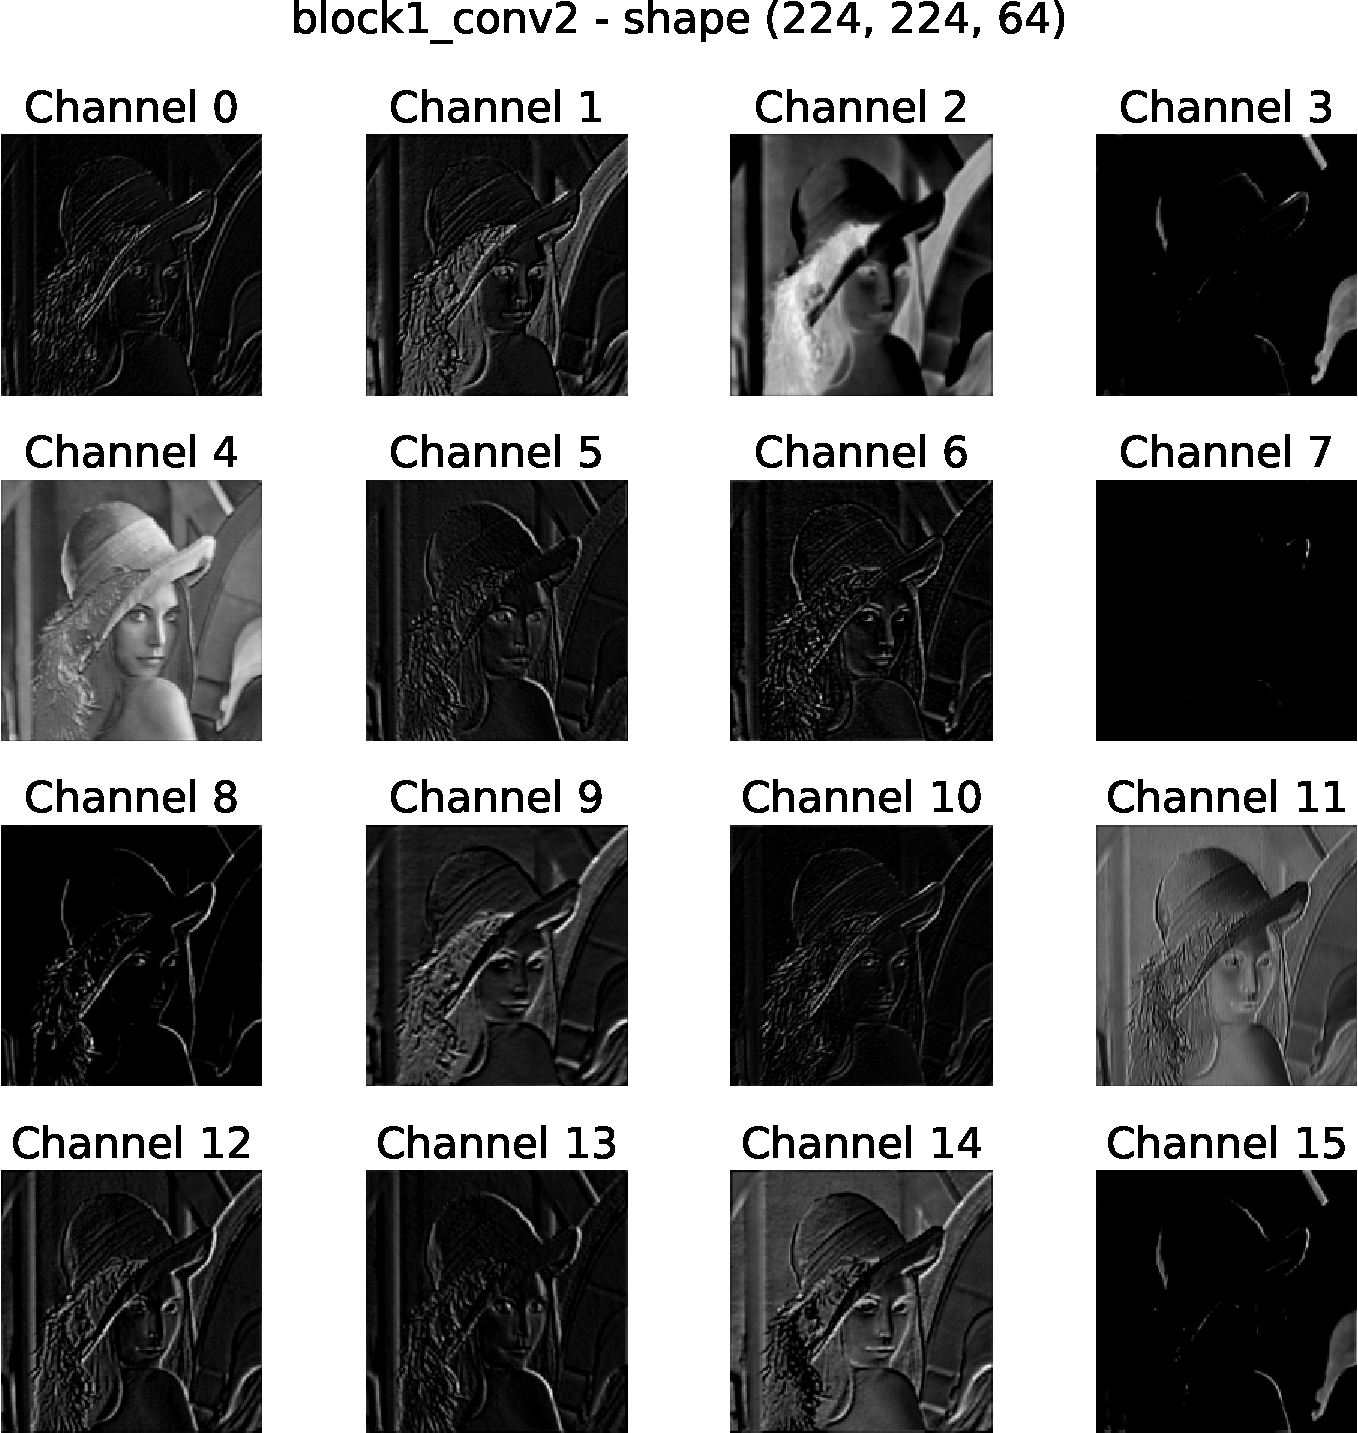
\includegraphics[width=.67\textwidth]{img/cnn/activations-block1_conv2.pdf}
    \caption{Activations produced by the first convolutional layer of VGG16 for the Lena image.}
    \label{fig:activations-block1_conv2}
\end{figure}

\noindent
\textcolor{Green3}{\faIcon{project-diagram} \textbf{Middle layers: combinations of features.}} Then look at the activations produced by the second convolutional layer of VGG16 for the Lena image in \autoref{fig:activations-block2_conv2}, and especially the third convolutional layer in \autoref{fig:activations-block3_conv3}. Something interesting happens: Lena becomes \textbf{progressively harder to recognize}.

\highspace
In \autoref{fig:activations-block2_conv2}, many channels still look like edges and textures, but in \autoref{fig:activations-block3_conv3}, the channels look more like abstract patterns. This is intentional because deeper layers are no longer asking only questions such as ``\emph{is there an edge here?}''; they can respond to \textbf{combinations of simpler features} detected in previous layers.

\highspace
Notice also that a filter in block 3 is \textbf{not operating directly on Lena's RGB pixels anymore}. It receives the feature maps generated by the preceding network layers as input.

\newpage

\begin{figure}[!htp]
    \centering
    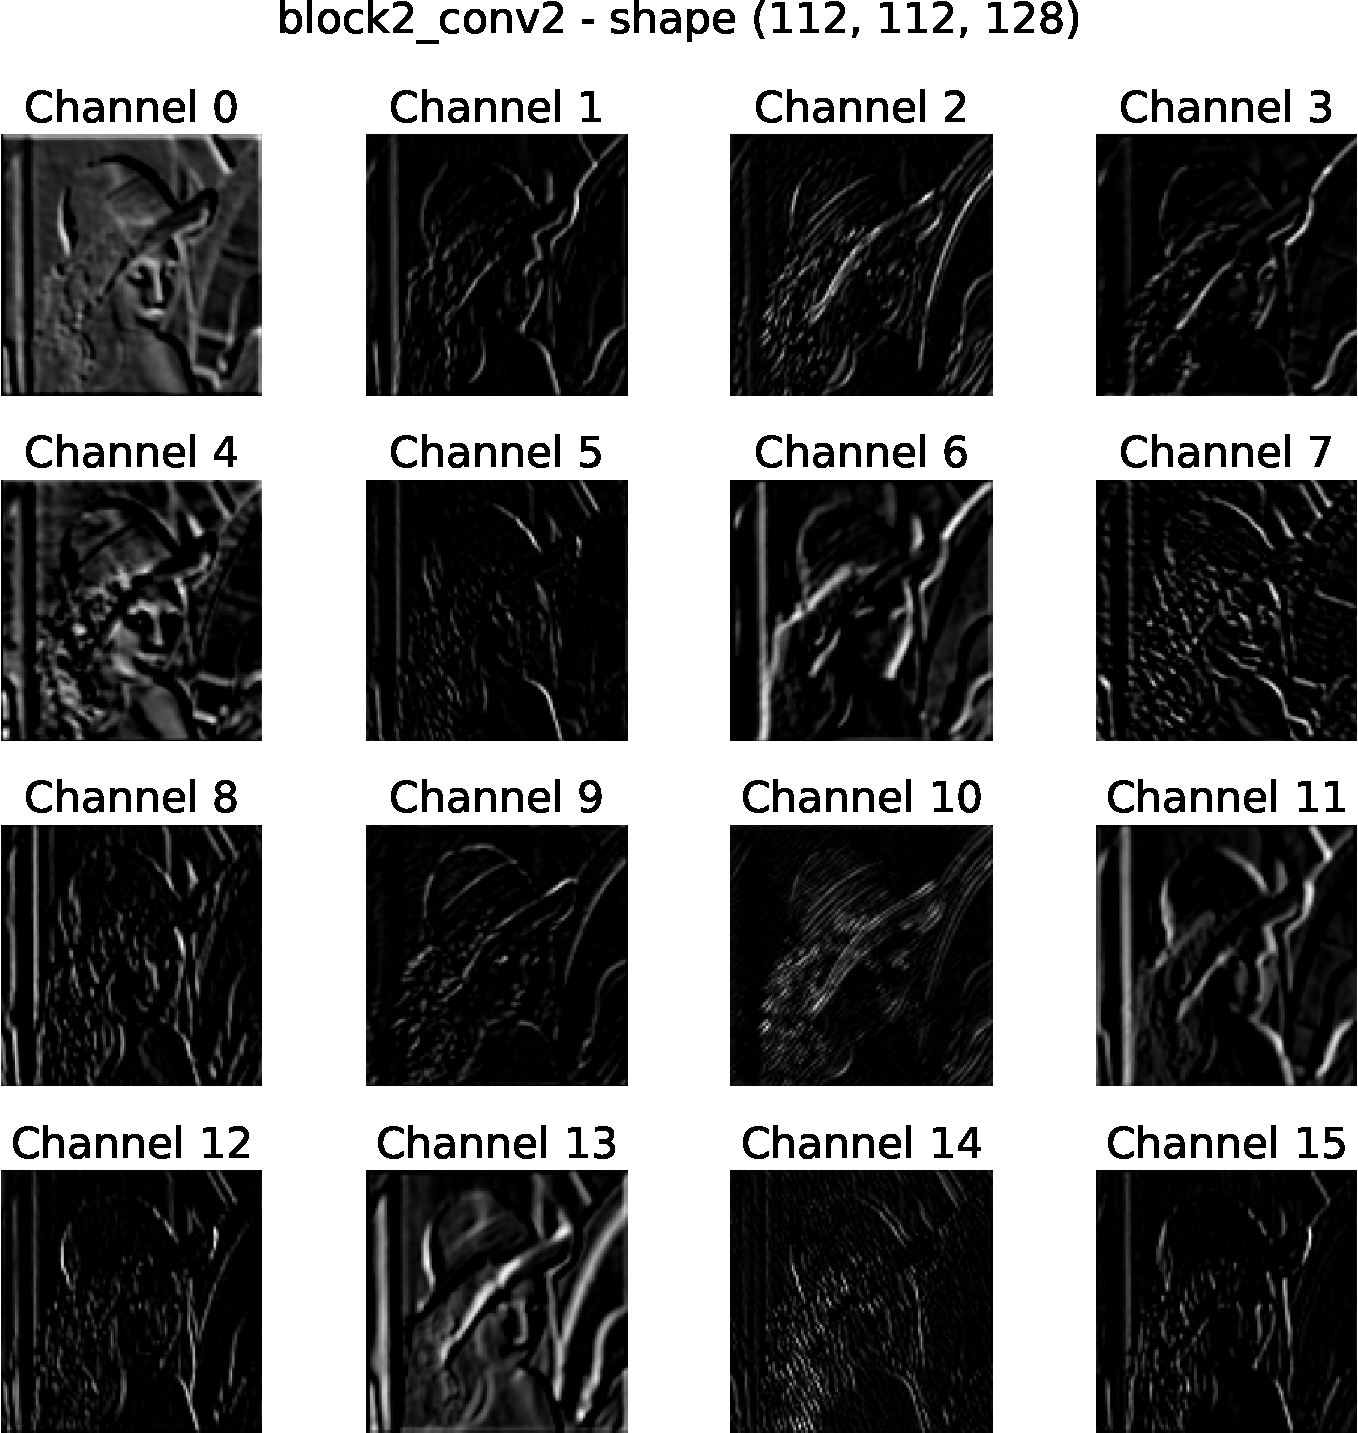
\includegraphics[width=.67\textwidth]{img/cnn/activations-block2_conv2.pdf}
    \caption{Activations produced by the second convolutional layer of VGG16 for the Lena image.}
    \label{fig:activations-block2_conv2}
\end{figure}

\begin{figure}[!htp]
    \centering
    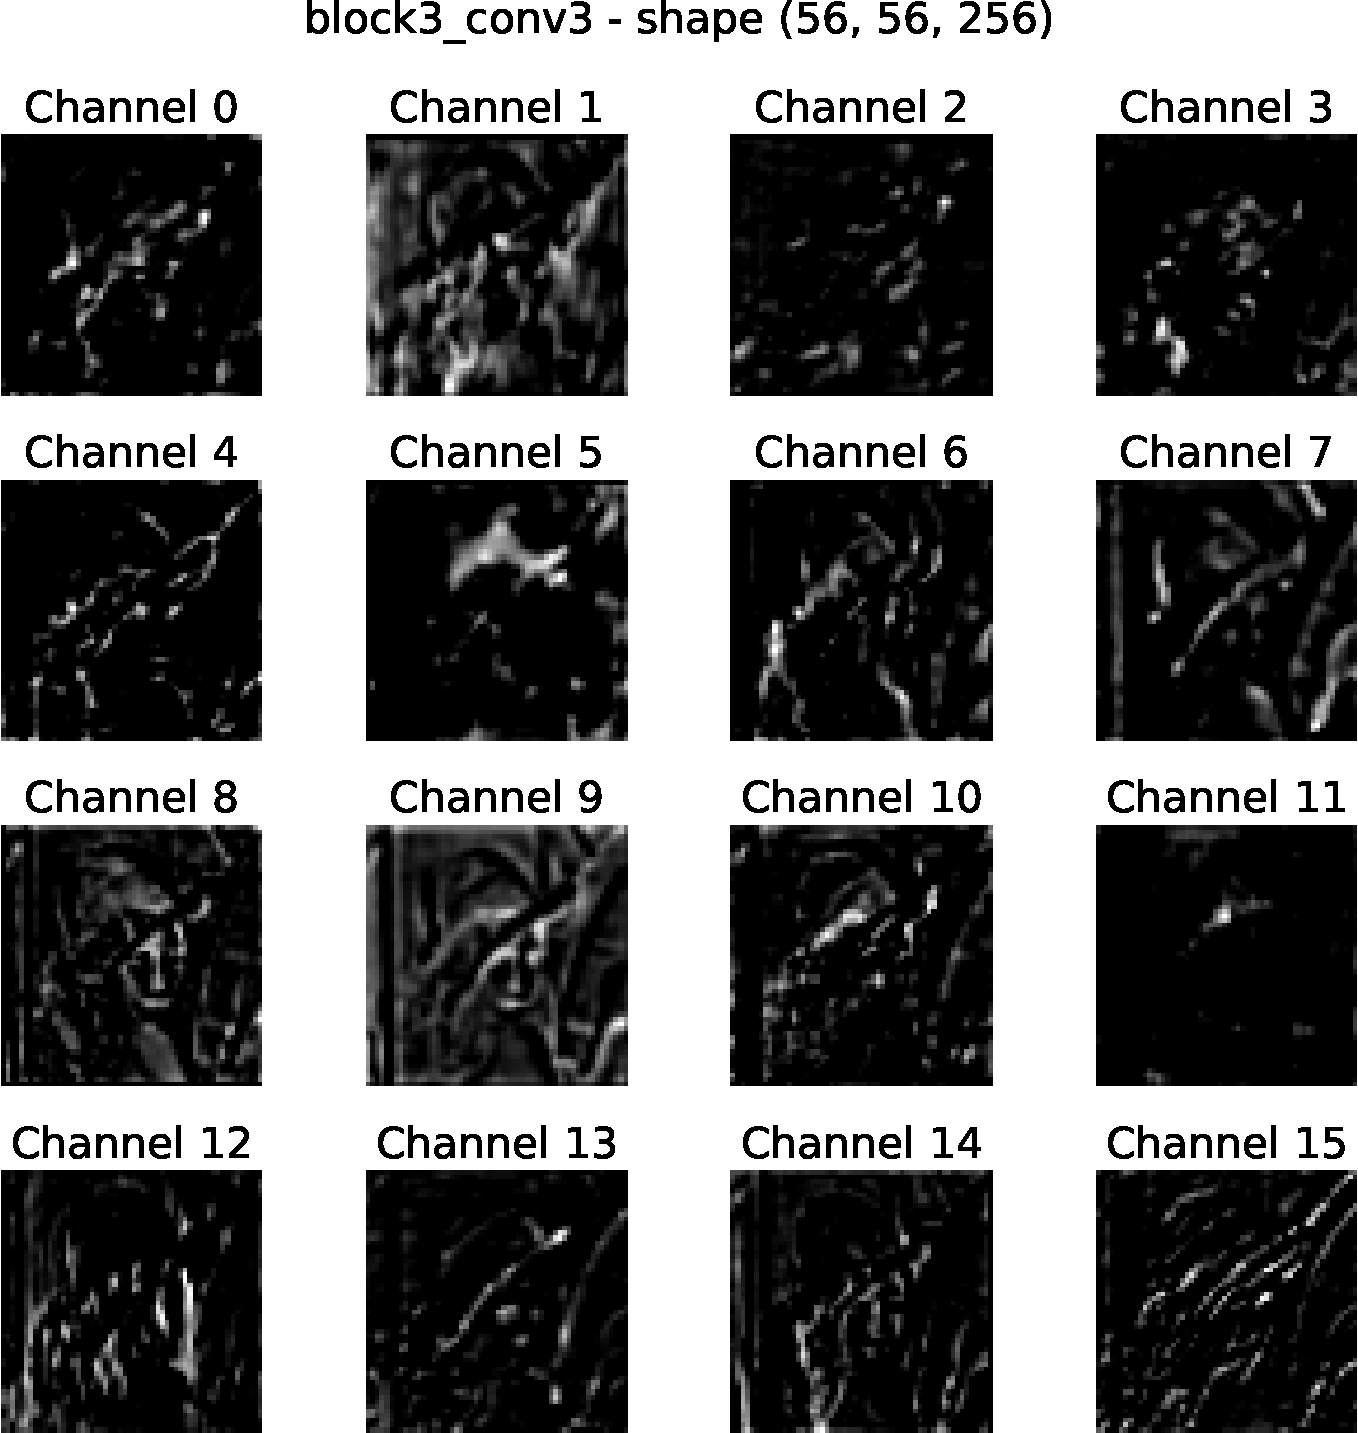
\includegraphics[width=.67\textwidth]{img/cnn/activations-block3_conv3.pdf}
    \caption{Activations produced by the third convolutional layer of VGG16 for the Lena image.}
    \label{fig:activations-block3_conv3}
\end{figure}

\newpage

\noindent
\textcolor{Green3}{\faIcon{braille} \textbf{Deep layers: sparse, abstract activations.}} Finally, look at the activations produced by the fourth convolutional layer of VGG16 for the Lena image in \autoref{fig:activations-block4_conv3} and the fifth convolutional layer in \autoref{fig:activations-block5_conv3}. 

\highspace
Many channels are almost completely black, with only a few strongly activated regions. That does \textbf{not} mean that the CNN has progressively ``\emph{lost}'' the image in a bad way. Rather, its representation has changed from something like ``\emph{what are the pixel values?}'' toward something like ``\emph{which learned high-level patterns are present, and approximately where?}''.

\highspace
For example, suppose some hypothetical deep feature $A_{137}$ has learned to respond strongly to a particular complex visual pattern. Then only locations containing something similar to that learned pattern produce large activations:
\begin{equation*}
    A_{137}(r, c) = \begin{cases}
        \text{large}        & \text{feature strongly present around location } (r, c) \\
        \text{small / 0}    & \text{otherwise}
    \end{cases}
\end{equation*}
This explains those little bright blobs in the \autoref{fig:activations-block5_conv3}.

\highspace
\textcolor{Red2}{\faIcon{exclamation-triangle} \textbf{One caution about interpretation.}} We should \textbf{not look at one of those blobs and claim}: ``\emph{Ah, that blob is the nose!}'' or ``\emph{That blob is the eye!}''. Because the visualization alone doesn't establish exactly what semantic concept a particular channel represents. What we \emph{can} safely say is that deeper channels respond selectively to increasingly complex patterns learned during training.

\highspace
\begin{takeawaysbox}[: Hierarchical feature learning]
    Each channel of a convolutional volume is a separate feature map and can be visualized as a grayscale image. Bright locations indicate where that learned feature produces a strong activation.

    \highspace
    Early CNN layers preserve fine spatial information and typically respond to simple visual patterns such as edges and textures. Deeper layers combine features produced by previous layers, producing increasingly complex and abstract representations. Consequently, the original image becomes progressively less recognizable when individual deep feature maps are visualized.

    \highspace
    Through the network, spatial resolution generally decreases while the number of feature channels increases:
    \begin{equation*}
        H, W \; \downarrow \quad \text{and} \quad C \; \uparrow
    \end{equation*}
    Thus, CNNs progressively transform raw pixels into a collection of learned, increasingly abstract visual features.
\end{takeawaysbox}

\newpage

\begin{figure}[!htp]
    \centering
    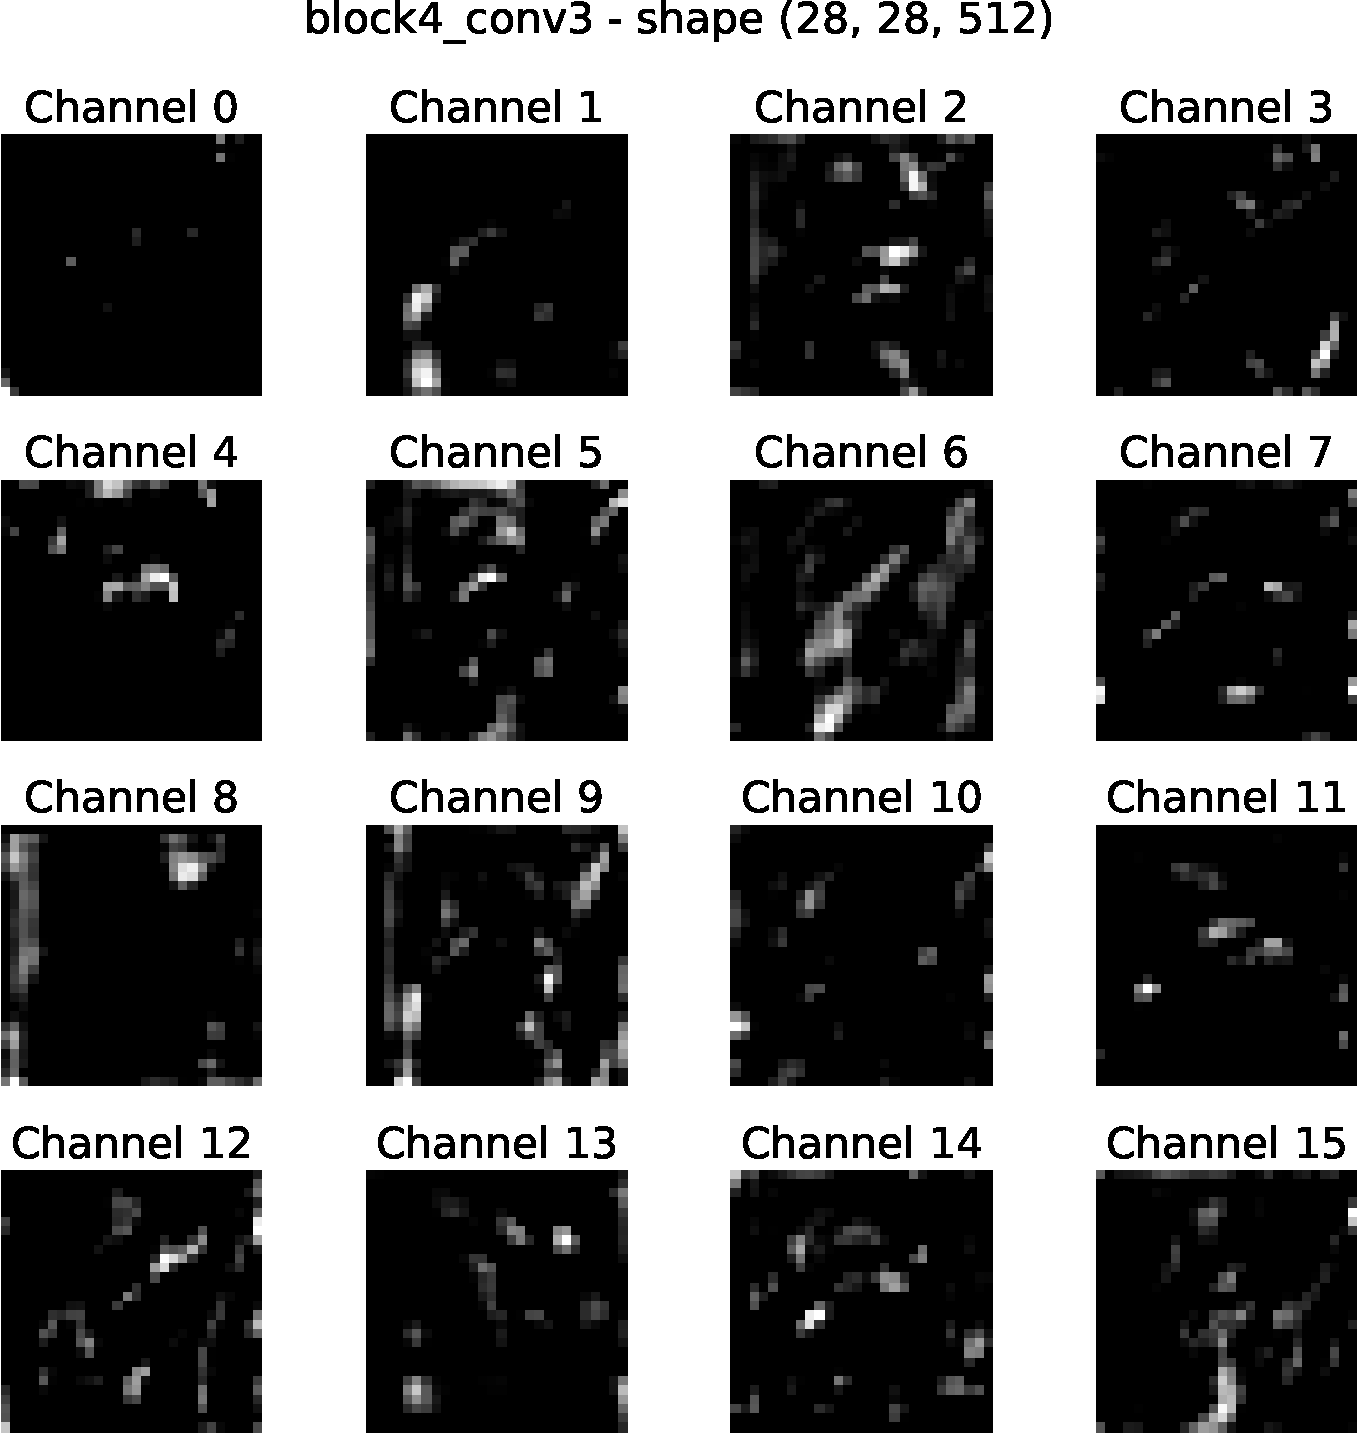
\includegraphics[width=.67\textwidth]{img/cnn/activations-block4_conv3.pdf}
    \caption{Activations produced by the fourth convolutional layer of VGG16 for the Lena image.}
    \label{fig:activations-block4_conv3}
\end{figure}

\begin{figure}[!htp]
    \centering
    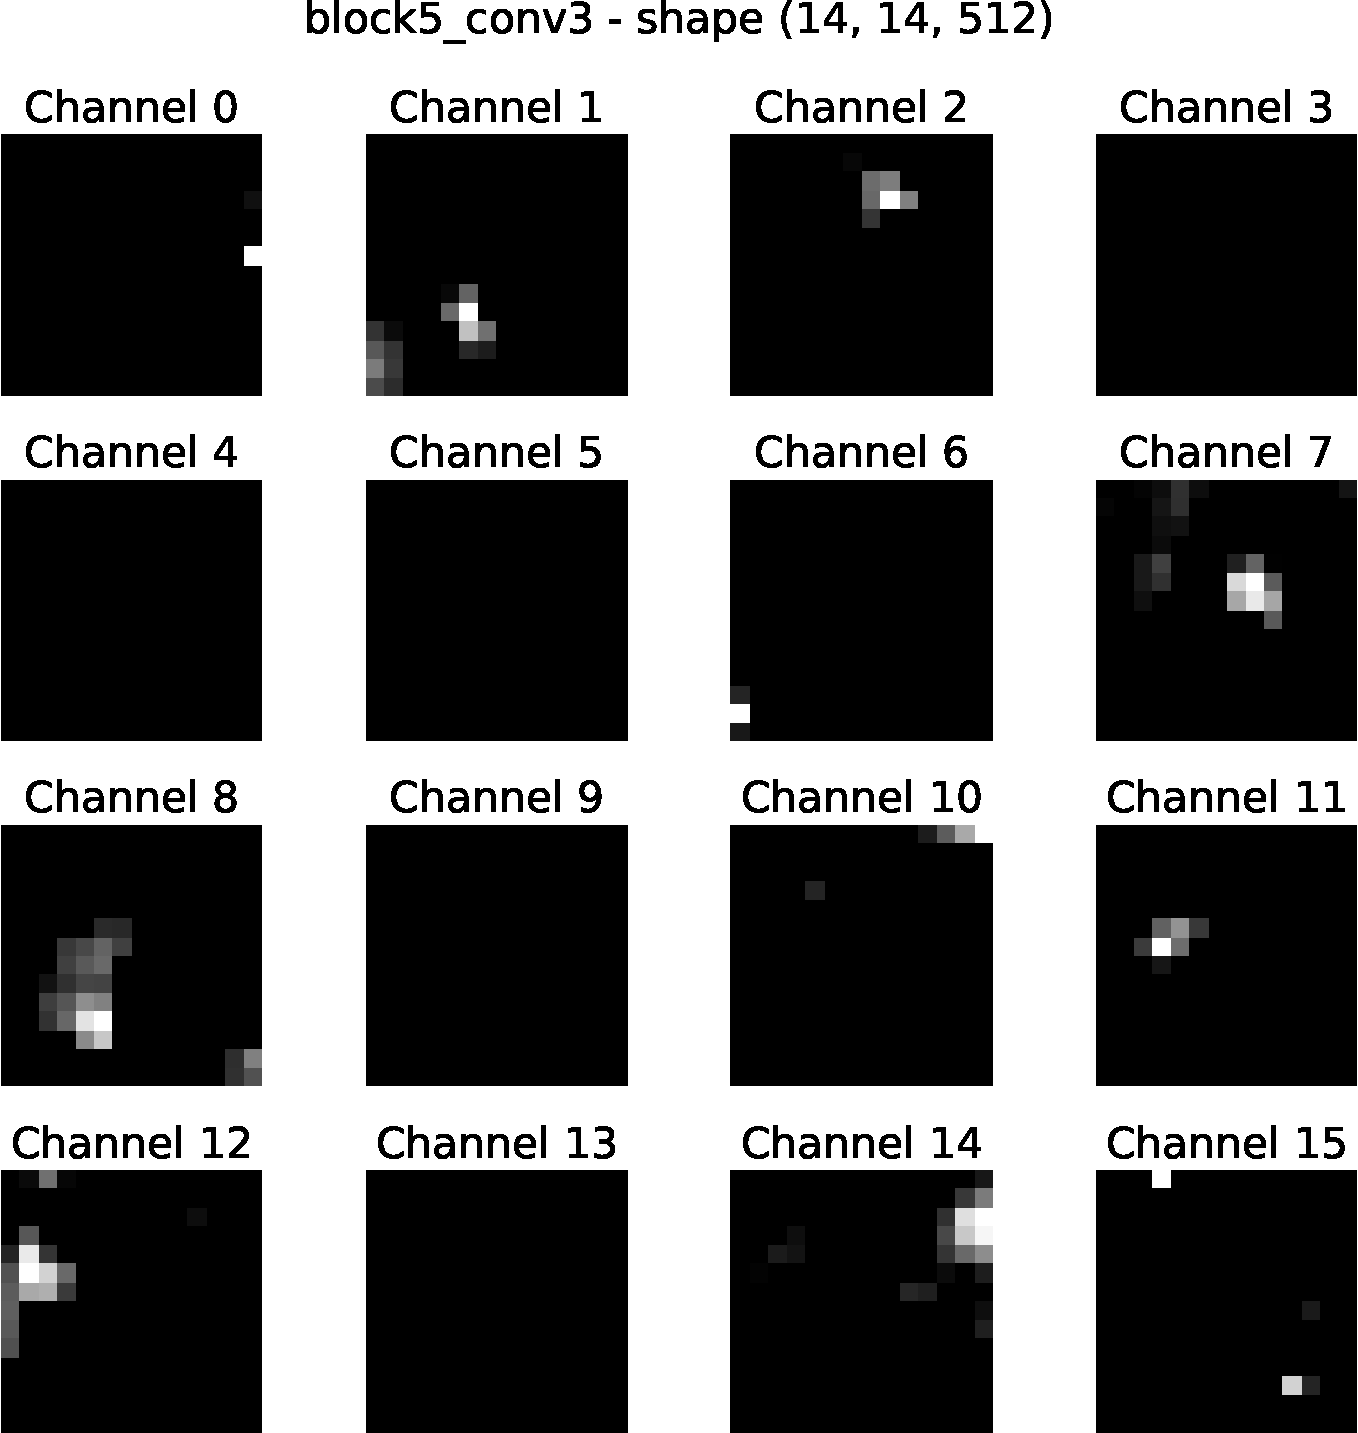
\includegraphics[width=.67\textwidth]{img/cnn/activations-block5_conv3.pdf}
    \caption{Activations produced by the fifth convolutional layer of VGG16 for the Lena image.}
    \label{fig:activations-block5_conv3}
\end{figure}